\subsection{A Network-based End-to-End Trainable Task-oriented Dialogue System \cite{Wen2016}}
The task is to help humans find a desired restaurant and the contact information from a database by conversing naturally with them. The paper proposes an end-to-end trainable framework for task-oriented systems shown in Figure \ref{fig:Wen2016Network01}.

\begin{figure}[htbp]
  \centering
  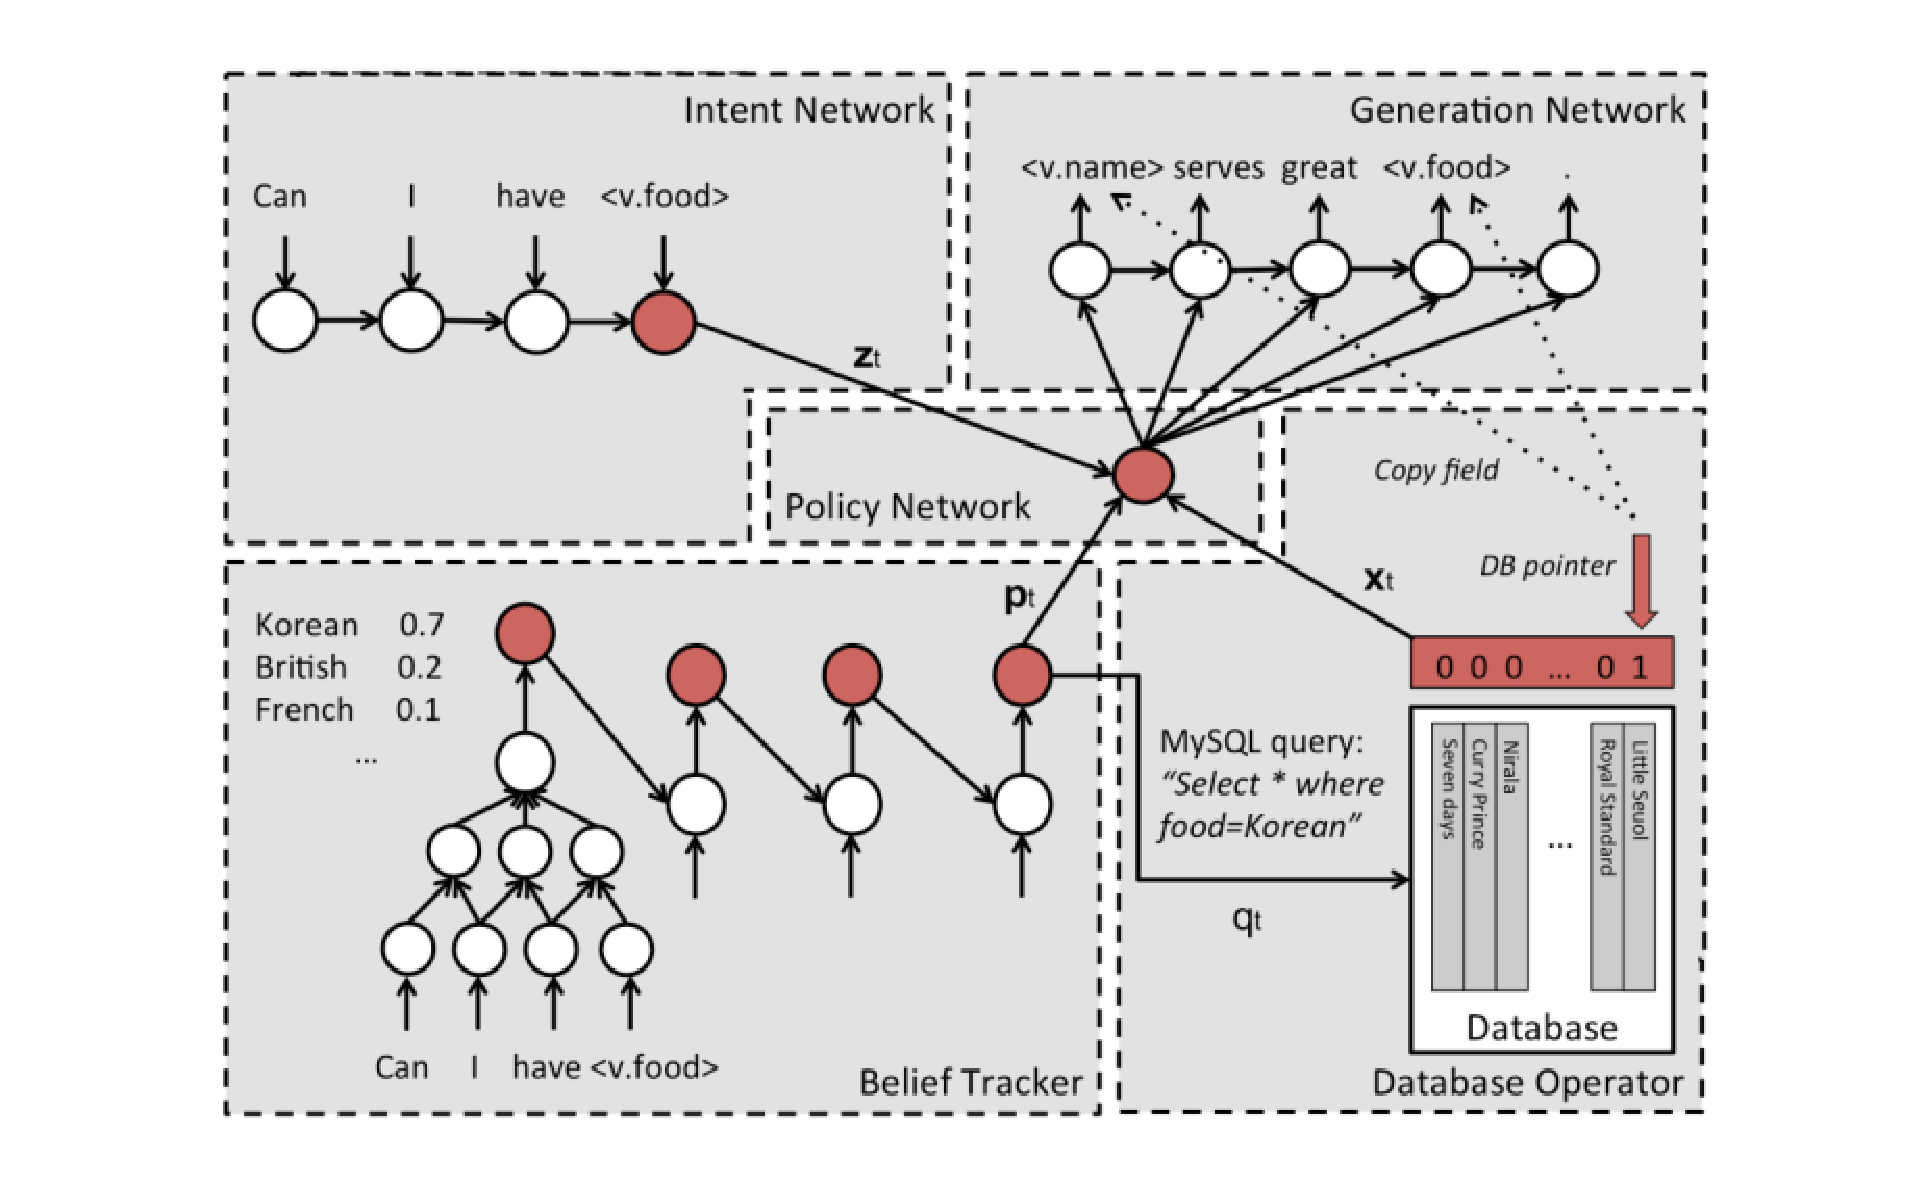
\includegraphics[width=0.9\linewidth]{Wen2016Network01}
  \caption{An end-to-end trainable framework for task-oriented systems}
	\label{fig:Wen2016Network01}
\end{figure}

At each turn, the system takes an user utterance $u^{t}$ as input, which is used to update two internal representations by an intent network and a set of belief trackers: (1) A distributed representation; (2) A distribution over the values, belief state, for each slot. The database operator uses the most likely values in the belief state, and returns the matched restaurants in the database. The policy network combines the distributed representation, belief state, and search results to form an action vector representing the next action. Conditioned on the action vector, the generation network produces template-like sentences whose generic tokens are then replaced by the actual values. Each components are described in more detail below:

\begin{itemize}
\item[-] \textbf{Intent Network} encodes $u^{t}=w^{t}_{0}, ..., w^{t}_{N}$ into a distributed representation $z^{t}$ at turn $t$. a LSTM is used and the last hidden state $z^{t}_{N}$ is taken as the distributed representation:
\begin{equation}
z^{t} \ = \ z^{t}_{N} \ = \ LSTM( w^{t}_{0}, ..., w^{t}_{N} )
\end{equation}

\item[-] \textbf{Belief Trackers} maintain a multinomial distribution $p^{t}_{s}$ for each informable slot and a bernoulli distribution $p^{t}_{s}$ for each requestable slot. The distributions are updated by:
\begin{equation}
\begin{aligned}
f^{t}_{s}(v) \ =& \ f^{t}_{s}(v,cnn) \oplus p^{t-1}_{s}(v) \oplus p^{t-1}_{s}(\emptyset) \\
g^{t}_{s}(v) \ =& \ U_{s} sigmoid( W_{s}f^{t}_{s}(v) + B_{s} ) + D_{s} \\
p^{t}_{s}(v) \ =& \ \frac{\exp(g^{t}_{s}(v))}{\exp(g^{t}_{s}(\emptyset)) + \sum_{v} \exp(g^{t}_{s}(v))} \\
\end{aligned}
\end{equation}
where $f^{t}_{s}(v)$ is the concatenation of two CNN feature vectors, one from processing $u^{t}$ and the other from processing the last action $a^{t-1}$.

\item[-] \textbf{Database Operator} forms a query
\begin{equation}
q^{t} \ = \ \cup_{s} { argmax_{v} p^{t}_{s}(v) }
\end{equation}
and create a binary vector $x^{t}$ over the restaurants in the database where a 1 means that the corresponding restaurant is consistent with the query.

\item[-] \textbf{Policy Network} outputs an action vector $o^{t}$ by:
\begin{equation}
o^{t} \ = \ \tanh( W_{z} z^{t} + W_{p} \oplus_{s} \hat{p}^{t}_{s} + W_{x} \hat{x}^{t} )
\end{equation}
where $\hat{p}^{t}_{s}$ is the belief summary consisting of (1) the summed value probabilities; (2) the probability that the user do not care; (3) the probability that the slot has not been mentioned, and $\hat{x}^{t}$ is a 6-bin 1-hot encoding vector based on the number of matched restaurants in $x^{t}$.

\item[-] \textbf{Generation Network} generates templates token by token conditioned on the action vector:
\begin{equation}
P(w^{t}_{i+1} | w^{t}_{i}, h^{t}_{i-1}, o^{t}) \ = \ LSTM( w^{t}_{i}, h^{t}_{i-1}, o^{t} )
\end{equation}
Instead of conditioning on a single action vector $o^{t}$, an attention mechanism can also be used to produce templates.

\end{itemize}